\section{On types and locality}\label{sec:gaifman}
In this section, we define the notion of types 
and prove a locality property, \cref{lem:types}.
We begin by recalling some standard notions from logic.

\subsection{Logical notions}


%
%
%
% extract from Gaifman's Locality Theorem~\cite{gaifman1982local} a technical lemma
% (\cref{pro:crossing} below), which will be used later in two different settings: in the proofs of \cref{thm:vc-density} and of \cref{thm:uqw-stable}.

\paragraph{Formulas}
All formulas in this paper are first order formulas,
i.e., they are built from variables (denoted $x,y,z$, etc.)
atomic predicates $x=y$ or $E(x,y)$,
denoting the existence of an edge between two nodes, using quantifiers $\forall x,\exists x$, boolean connectives $\lor,\land,\neg$. 
Let $\phi(\bar x)$ is a formula with free variables 
$\bar x$. (Formally, the free variables form a set.
To ease notation, we identify this set with a tuple by fixing any its enumeration.)
If $\bar w\in V^{|\bar x|}$ is a tuple of vertices of some graph $G=(V,E)$ (treated as a valuation of the free variables $\bar x$), then we write $G,\bar w\models \phi(\bar x)$
to denote that the valuation $\bar w$ satisfies the formula $\phi$ in the graph $G$.
The following example should clarify our notation.

\begin{example}\label{ex:dist-formula}
The formula
$$\phi(y,z)\equiv \exists x_1.\exists x_2. (E(y,x_1)\lor (y=x_1))\land (E(x_1,x_2)\lor (x_1=x_2))\land (E(x_2,z)\lor (x_2=z))$$
with free variables $y,z$ expresses that $y$ and $z$ are at distance at most $3$, 
i.e., for two vertices $u,v$ of a graph $G$,
the relation $G,u,v\models \phi(y,z)$ holds 
if and only if the distance between $u$ and $v$ is at most $3$ in $G$.
\end{example}

We will consider also \emph{colored graphs},
where every vertex can be assigned a set of colors from 
a fixed set of colors. If $C$ is a color then the formula $C(x)$ holds in a vertex $x$ if and only if $x$ has color $C$.

Finally, we will consider \emph{formulas with parameters}
from a set  $A$ which is a set of vertices of some graph.
Such a formula is formally a formula $\phi(\bar y,\bar z)$
with a partitioning of its free variables into two sets $\bar y$ and $\bar z$,
and a valuation $\bar w\in A^{|\bar z|}$ of the free variables $\bar z$ in $A$. 
We denote the resulting formula with parameters by $\phi(\bar y,\bar w)$, and say that its free variables 
are $\bar y$. For a valuation $\bar u\in A^{|\bar y|}$,
we write $G,\bar u\models \phi(\bar y,\bar w)$
if $G,\bar u\bar w\models \phi(\bar y,\bar z)$.



% Occasionally, we will consider additional atomic predicates over an extended vocabulary. In such cases, we will explicitly specify the vocabulary.
% \paragraph{Valuations}
% Let $\phi(\bar x)$ be a formula with  free variables $\bar x$.
% We remark that although it is customary to treat free variables
% as \emph{tuples}, it is in fact more convenient to treat them as \emph{sets}
% (in particular, they are non-repeating). In what follows,
%  we formally consider \emph{sets} of free variables of a formula, despite of the notation $\bar x$.
%  Sets of free variables will be denoted by the symbol $\bar x,\bar y, \bar z$.
% The concatenation $\bar x\bar y$ denotes the union of the sets $\bar x$ and $\bar y$.
%
%  Let $G=(V,E)$ be a graph.
%  If $A\subset V$ is a set of vertices, then
% by $A^{\bar x}$ we denote the set of \emph{valuations}
% of the variables $\bar x$ in $A$, i.e.,
% functions $\bar u\from \bar x\to A$. Clearly, a valuation can be identified with a tuple of elements of $A$ of length $|\bar x|$.
% Note  that unlike $\bar x$,
% a valuation $\bar u$ is a function, not a set. In particular,
% $\bar u$ may contain repetitions, in the sense that
% it may map several variables to the same element in $A$.
% To avoid confusion, by $\bar x,\bar y,\bar z$ we will always mean
% sets of variables, whereas $\bar u,\bar v,\bar s$ will denote valuations. A valuation $\bar u$ does not have to be considered in the context of a formula, but it always has an underlying tuple $\bar x$, which is the domain of $\bar u$.
% Write $G,\bar u \models \phi(\bar x)$ to denote
% that the formula $\phi$ holds in the graph $G$, under the valuation $\bar u$ of the variables $\bar x$.
% We omit the usual Tarski'an recursive definition.


\paragraph{Types}
\newcommand{\tp}{\mathrm{tp}}
% We first define formulas with \emph{parameters} from a set of vertices.
Fix a formula $\phi(\bar y,\bar z)$ together with a distinguished partitioning of its free variables into 
\emph{object variables} $\bar y$ and \emph{parameter variables} $\bar z$. 
% , called the \emph{object} variables and the \emph{parameter} variables, respectively.
Let $G=(V,E)$ be a graph, $A\subset V$.
% By $\phi(\bar y,\bar v)$ we formally mean the
% pair $(\phi(\bar y,\bar z),\bar v)$,
% We call $\phi(\bar y,\bar v)$  a \emph{formula with parameters from $A$}.
% % or to be more specific, an \emph{instance} of $\phi(\bar y,\bar z)$ with parameters from $A$.
% If $\bar u\in V^{\bar x}$ is a valuation of $\bar y$
% in $V$ then we write $G,\bar u\models \phi(\bar y,\bar v)$
% to denote that $G,\bar u\bar v\models \phi(\bar y,\bar z)$,
% where $\bar u\bar v\in V^{\bar x\bar y}$ is the valuation obtained as the set-theoretic union of $\bar u$ and $\bar v$.
% The set of free variables of $\phi(\bar y,\bar v)$ is $\bar y$, and its \emph{quantifier rank}
% is  the quantifier rank of $\phi(\bar y,\bar z)$
% (i.e., the maximal nesting of quantifiers).
If $\bar u\in V^{|\bar y|}$ is a tuple of 
nodes of length $|\bar y|$, then the 
\emph{$\phi$-type of $\bar u$ over $A$},
denoted $\tp^\phi_G(\bar u/A)$,
is the set of all
formulas  $\phi(\bar y,\bar v)$ 
with parameters $\bar v$ from $A$
replaced by the parameter variables $\bar z$,
such that $G,\bar u\models \phi(\bar y,\bar v)$.
Therefore, up to  bijection, we have the following identification:
$$\tp^\phi_G(\bar u/A)\quad\leftrightarrow\quad\setof{\bar v\in  A^{|\bar z|}}{G, \bar u\bar v\models \phi(\bar y,\bar z)}.$$
% In other words, $\tp^\phi_G(\bar u/A)$ corresponds to the
% neighborhood of $\bar u\in V^{|\bar y|}$ in the bipartite graph with parts $V^{|\bar y|}$ and $A^{|\bar z|}$,
% and edge relation defined by $\phi(\bar y,\bar z)$.


If $q\in \N$ is a number and $\bar u\in  V^{d}$
is a tuple of some length $d$, then by $\tp^q_G(\bar u/A)$  we denote the set of all formulas $\phi(\bar y,\bar v)$
of quantifier rank $q$ with parameters $\bar v$ from $A$,
such that $G,\bar u\models \phi(\bar y,\bar v)$.
Therefore, up to  bijection, we have the following identification:
$$\tp^q_G(\bar u/A)\quad\leftrightarrow\quad\set{tp^\phi(\bar u/A)}_{\phi(\bar y,\bar z)},$$
where $\phi(\bar y,\bar z)$ ranges over all formulas of quantifier rank $q$, and all partitions of its free variables into two sets $\bar y,\bar z$,
where $|\bar y|=d$. 
In particular, the set $\tp^q_G(\bar u/A)$ is infinite.
It is not difficult to see, however, that in the case when $A$ is finite,
the set $\tp^q_G(\bar u/A)$ is uniquely determined by its finite subset, since up to syntactic equivalence, there are only finitely many formulas of quantifier rank $q$ with $|\bar u|$ free variables and  parameters from $A$
(we can assume that each such formula has $|A|+|\bar u|$ free variables).
Moreover, the set of all possible types 
$\tp^q_G(\bar u/A)$ is bounded by some number 
depending in a computable way only from 
$q,|\bar u|$ and $|A|$.

% This could be used for providing a finite representation of a type. Another way is to represent a type as a blackbox algorithm (a Turing machine, if you will), which inputs a formula
% $\phi(\bar y,\bar w)$ with parameters $\bar w$ from $A$ and outputs \emph{yes} or \emph{no}, depending on whether
% $\phi(\bar y,\bar w)$ belongs to the type. We will use this representation.




 % (however, it can be described in a finite way
% if $A$ is finite -- see
%  \cref{lem:fin-type} below).




 




% For a fixed numbers $q,d\in \N$, and $G,A,W$ as above,
% define
%  $S^{q}_d(W/A)$ as the set of all quantifier-rank $q$ types over $A$ in $G$ of $d$-tuples of vertices from $W$, i.e.,
% \begin{align*}
% S^{q}_d(W/A)&=\setof{\tp^q(\bar u/A)}{\bar u\in V^d}.
% \end{align*}
% In case $W=V(G)$ we write $S^{q}_d(G/A)$ instead of
% $S^{q}_d(W/A)$.
% , although one can show that if the set $A$ is finite, then
% $\tp^q(\bar u/A)$ is uniquely determined by a finite subfamily of
% $\set{tp^\phi(\bar u/A)}_{\phi(\bar y,\bar z)}$
% (one can bound $|\bar z|$ by $|A|$
% and note that there are only finitely many  formulas $\phi(\bar y,\bar z)$ of quantifier rank $q$, up to semantic equivalence).

In  case when $\Delta$ is either a formula $\phi(\bar y,\bar z)$ with a distinguished partitioning of its free variables, or a number $q$,
we simply write $\tp^\Delta(\bar u/A)$ if the graph $G$
is clear from the context. %, or  write $\tp^\Delta[G,\bar u, A]$
%if the graph $G$ needs to be explicated. 
In the case $A=\emptyset$, we omit it from the notation, 
and simply write $\tp^\Delta(\bar u)$ or $\tp^\Delta_G(\bar u)$.

\begin{example}
Let $\phi(y,z)$	be the formula from~\cref{ex:dist-formula}, denoting that the distance between $y$ and $z$ is at most $3$.
We  partition  the free variables of $\phi$
into $y$ and $z$.
Let $A$ be a set of vertices of a graph $G=(V,E)$
and $u\in V$ be a single vertex.
The $\phi$-type of $u$ over $A$
corresponds to the set of those vertices in $A$
whose distance from $u$ is at most $3$ in $G$.
% It is not difficult to construct examples of graphs $G$
% and subsets $A$ for which $|S^\phi(G/A)|=2^{|A|}$.
% Indeed, for the formula considered above,
% pick any set $A$ and for each subset $B\subset A$
% create a vertex $v_B$ which is adjacent to every vertex in $B$. Let $G$ be the resulting graph, with every edge
% replaced by a path of length $3$. Then $\tp^\phi(v_B/A)$
% corresponds to the subset $B$ of $A$, i.e.,
% $\tp^\phi(v_B/A)$ is  the set of formulas $\phi(y,b)$,
% for all $b\in B$. Since $B$ ranges over all subsets of $A$,
% we get that $|S^\phi(G/A)|=2^{|A|}$.
\end{example}


For a fixed formula $\phi(\bar y,\bar z)$,  graph $G=(V,E)$ and sets $A,W\subset V$, define
 $S^\phi(W/A)$ as the set of all $\phi$-types of tuples from $W$ over $A$ in $G$
i.e., \begin{align*}
S^\phi(W/A)&=\setof{\tp^\phi_G(\bar u/A)}{\bar u\in W^{|\bar y|}}.
\end{align*}
Although not visible in the notation, the set $S^\phi(W/A)$ depends on the chosen partitioning $\bar y,\bar z$ of the free variables of $\phi$.
In case $W=V(G)$ we write $S^{\phi}_d(G/A)$ instead of 
$S^{\phi}_d(W/A)$.

The following lemma is immediate.
\begin{lemma}\label{lem:types-over-B}
Let $G$ be a graph and let $A\subseteq B\subseteq V(G)$. Then 
$|S_\phi(G/A)|\leq |S_\phi(G/B)|$. 
\end{lemma}
% \begin{proof}
% Observe that whenever $\tp^\phi(\tup v/A)\neq \tp^\phi(\tup w/A)$, we also have $\tp^\phi(\tup v/B)\neq \phi(B,\tup w)$.
% \end{proof}


% The following simple lemma shows that if the set of parameters $S$ has bounded size, then the type $\tp^q(\bar u/S)$ only contains a bounded amount of information.
% \begin{lemma}\label{lem:fin-type}Let $q,d,s$ be  numbers.
%   There is a finite set of formulas $\cal F$  formulas of the form
%   $\phi(\bar y,\bar z)$ with $|\bar y|=q,|\bar z|=s$, and of quantifier rank $q$
%   such that for every graph $G=(V,E)$,
%   set $S\subset V$ with $|S|\le s$
%   and  $\bar u\in V^d$, the type $\tp^q(\bar u/S)$ is uniquely determined by   $\set{\tp^\phi(\bar u/S)}_{\phi(\bar y,\bar z)\in\cal F}$.
%   The set $\cal F$ is computable from $q$ and $s$.
%   In particular, $|S^{q}_d(G/S)|\le T(q,d,s)$,
%   for some computable function $T\from \N\times \N\times\N\to \N$.
% \end{lemma}
% \begin{proof}[Sketch of proof]
%   Take ${\cal F}_0$ to be the set of all formulas of the form $\phi(\bar y,\bar z)$
%   (where $\bar y$ and $\bar z$ are  as in the statement) and of quantifier rank $q$. Up to syntactic equivalence,  ${\cal F}_0$
%   contains only finitely many elements.
%   Let ${\cal F}\subset {\cal F}_0$ be a finite set of representatives of ${\cal F}_0$, up to syntactic equivalence.
% Then $\cal F$ satisfies the required conditions.
% \end{proof}



\subsection{Locality}
If $X,Y,S\subset V(G)$ are sets of vertices of a graph $G$ 
and $r\in \N$, then we say that $X$ and $Y$ are  \emph{$r$-separated}
by $S$  (in $G$) if every path between a vertex in $X$ and a vertex in 
$Y$ of length at most~$r$ contains a vertex from $S$ (cf.~Fig.~\ref{fig:sep}).

\begin{figure}[h!]
	\centering
		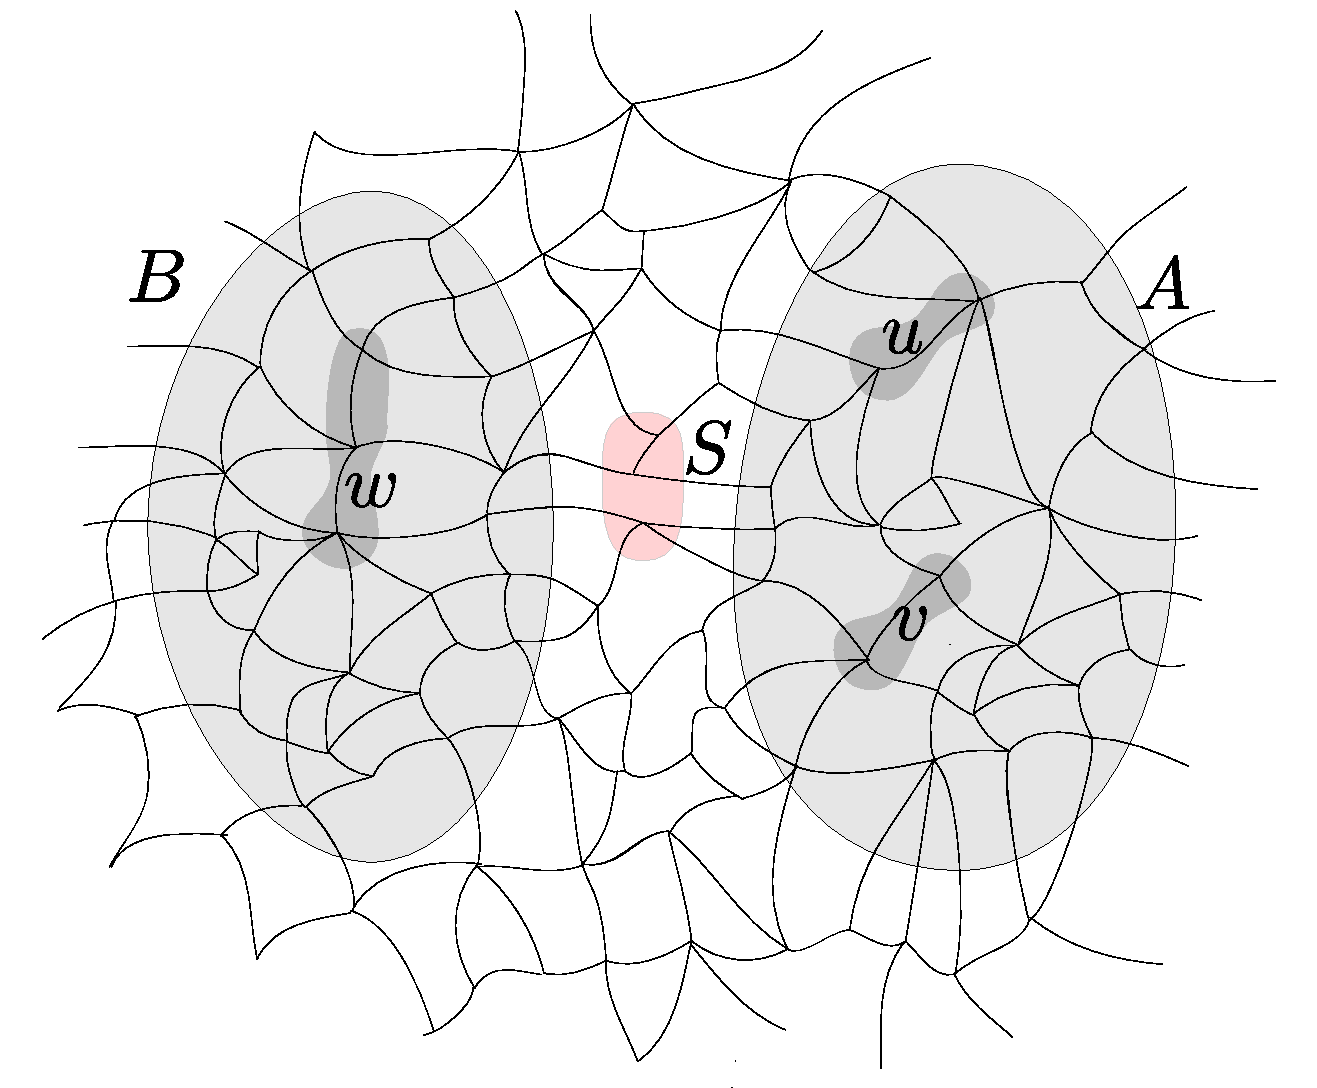
\includegraphics[scale=0.35,page=1]{pics}
	\caption{The sets $A$ and $B$ are $2$-separated by $S$.
	}
	\label{fig:sep}
\end{figure}

% If $\bar u\in V^{\bar y}$ is a valuation of some set of variables $\bar y$ in a set $V$, then we say
% that $X$ and $\bar y$ are $r$-separated by $S$
% if $X$ and $Y$ are $r$-separated by $S$, where $Y$ is the range of $\bar y$.

%  If $G$ is a graph, $B\subset V(G)$ is a set of vertices,
% and $u,v\in V(G)^d$ are two tuples of vertices, then we say that
% $u$ and $v$ have \emph{the same quantifier rank $q$ type} over $B$
% if $u$ and $v$ satisfy exactly the same formulas of quantifier rank $q$ with parameters from $B$.
% Precisely,
% for every $k\in \N$, every tuple $u\in B^{k}$ of $k$ elements of $B$, and every formula $\phi$ of quantifier rank $q$ and with $d+k$ free variables, we have that $\phi(u,w)$ holds if and only if $\phi(v,w)$ holds.

The following lemma is the main result of~\cref{sec:gaifman}.




\begin{lemma}%[Gaifman locality $\lor$ Feferman-Vaught]
	\label{lem:types}
For any given number $q$
one can compute numbers $p,r$ with the following properties.	For any graph $G=(V,E)$ and sets of vertices $A,B,S\subset V$	
	such that $A$  and $B$ are $r$-separated by~$S$,
	for every tuple $\bar u\in A^{d}$, 
	the type $\tp^q(\bar u/B)$
	is computable from  $\tp^{p}(\bar u/S)$, and $G$ and $S$.
 
  
    %
  % Moreover, there is a computable function $T\from \N\times\N\times\N\to\N$
  % such that $|\setof{\tp^{q}(\bar u/A)}{\bar u\in B^d}|\le T(q,d,|S|)$.
  %
  
		%
	% and any $\bar u,\bar v\in B^{\bar y}$, the following implication holds:
	% $$\text{if\quad}\tp^q(\bar u/S)=\tp^q(\bar v/S)\text{\quad then\quad}
	% 	\tp^q(\bar u/A)=\tp^q(\bar v/A).$$
\end{lemma}

We say that a tuple $\bar u$ of vertices  is $r$-\emph{separated} from $B$ by $S$ if its underlying set of vertices is $r$-separated from $B$ by $S$.

\begin{corollary}\label{cor:bound}
There is a number
  $T$ computable from $q,d$ and $s$
  such that for any $S\subset V(G)$ with $|S|\le s$
    and set $U\subset V(G)^d$
  of $d$-tuples, each of which is  $r$-separated from $B$ by $S$, the inequality 
     $|\setof{\tp^q(\bar u/B)}{u\in U}|\le T$ holds.
\end{corollary}

\cref{cor:bound}  follows from~\cref{lem:types} by taking  $A$ to be
the set of all vertices which occur in a tuple in $U$.
Since $q$ is computable from $p$
and that the number of quantifier rank $p$ types of $d$-tuples of elements over a set of parameters of  size $s$ is bounded by a value computable from $p,q,s$, the corollary follows. 




%
% Without the computability requirements,
% it is not  difficult to derive the above result from the compactness
% theorem for first order logic.
% \begin{proof}[non-effective variant; sketch]
% 	Fix a number $q\in\N$ and a set of variables $\bar y$. We show that there is a number $n\in\N$  such that for any graph $G=(V,E)$, sets of vertices $A,B,S\subset V$
% 	such that $A$  and $B$ are $r$-separated by $S$,
% 	and any $\bar u,\bar v\in B^{\bar y}$, the following implication holds:
% 	$$\text{if\quad}\tp^n(\bar u/S)=\tp^n(\bar v/S)\text{\quad then\quad}
% 		\tp^q(\bar u/A)=\tp^q(\bar v/A).$$
%
% 	Suppose for the sake of contradiction, that
% 	for every $n\in\N$
% 	there is a graph $G_n=(V_n,E_n)$, sets of vertices $A_n,B_n,S_n\subset V_n$ such that $A_n$ and $B_n$ are $n$-separated by $S_n$ in $G_n$, and
% 	valuations  $\bar u_n,\bar v_n \in B^{\bar y}$
% 	such that $\tp^n(\bar u/S)=\tp^n(\bar v/S)$,
% 	however, $\tp^q(\bar u/A)\neq \tp^q(\bar v/A)$.
% For simplicity, we assume that the graphs $G_n$ are finite.
%
% The  inequality $\tp^q(\bar u/A)\neq \tp^q(\bar v/A)$ implies that there is a formula $\phi_n(\bar y)$ with parameters from $A_n$ such that $G_n,\bar u\models\phi_n(\bar y)$ and $G_n,\bar u\models\neg\phi_n(\bar y)$.
%
% Consider a signature consisting of the binary relation symbol $E$, constant symbols $a_1,a_2,\ldots$
% and $\bar u^1,\ldots,\bar u^k,\bar v^1,\ldots,\bar v^k,$
% where $k=|\bar y|$,
%  and unary relation symbols $A, B, S$.
%
% 	Define a structure $\mathbb G_n$ over this signature as the graph $G_n$, extended additionally by the following interpretations:
% 	\begin{itemize}
% 		\item 	 the predicate $A$ is interpreted
% 	as the set $A_n$,
% 	\item  $B$ is interpreted as the set $B_n$,
% 	\item $S$ is interpreted as $S_n$,
% 	\item $u^i$ is interpreted as the $i$th element of
% 	the tuple $\bar u_n$ (under  fixed enumeration of $\bar y$),
% 	for $i=1,\ldots,k$,
% 	\item $v^i$ is interpreted as the $i$th element of
% 	the tuple $\bar v_n$	for $i=1,\ldots,k$,
% 	\item $a_1,a_2,\ldots$ is interpreted to be any sequence  of vertices which enumerates the set of parameters which occur in the formula $\phi_n$.
% 	\end{itemize}
%
% 	Then, the structure $\str G_n$
% 	satisfies the sentence $\phi_n'$ expressing the conjunction of following properties:
% 	\begin{itemize}
% 		\item The sets $A_n$ and $B_n$ are $n$-separated by $S_n$,
% 		\item The elements
% 	\end{itemize}
%
%
%
%
% \end{proof}


% In other words, the conclusion of the lemma says that whether a tuple $\bar u\in B^{\bar y}$ satisfies a formula of quantifier rank $q$ with parameters from $A$ depends only on $\tp^q(\bar u/S)$
% (and on $G$ and $S$).

\medskip The rest of~\cref{sec:gaifman} is devoted to the proof of~\cref{lem:types}.
The lemma is a consequence of Gaifman locality of first order logic and a Feferman-Vaught type  lemma, which we recall now.
\medskip

% For a valuation $\bar u\in A^{\bar x}$ and number $r\in \N$, denote by
% $N^r_G(\bar u)$ the subgraph of $G$ induced by the set of vertices whose distance from a vertex in (the range of) $\bar u$
% is at most $r$.


\begin{lemma}[Gaifman locality]\label{lem:gaif}
  Let $G=(V,E)$ be a graph colored by a fixed number of colors, $A\subset V$ a set of vertices and $d\in \N$ a number.
  Then, for every tuple $\bar u\in V^d$, the type  $\tp^q(\bar u)$ is computable from $G$ and $\tp^q(B^r(\bar u))$, where $r=7^q$.
\end{lemma}
\cref{lem:gaif} is an immediate corollary of the main result in the paper of Gaifman~\cite{gaifman1982local}.

% Note that~\ref{lem:gaif} is a special case of~\cref{lem:types}, for $s=0$ and $A,S=\emptyset$.

% \begin{lemma}\label{lem:fv}
%   Let $G=(V,E)$ and $H=(W,F)$ be two graphs with disjoint vertex sets.
%   Then, for valuations
%  $\bar u\in V^{\bar y}$ and $\bar v\in W^{\bar z}$,
% $\tp^q_{G\oplus H}(\bar u\bar v)$
%  depends only on
%  of $\tp^q_G(\bar u)$ and $\tp^q_H(\bar v)$.
% \end{lemma}
 % Let $G=(V,E)$ and $H=(W,F)$ be two graphs  with possibly non disjoint vertex sets. For a set $S$ we say that $G,H$
 % are $S$-\emph{touching} if $V\cap W\subset S$.
 %   In this case, by $G\cup_S H$
 % we denote the graph with vertex set $V\cup W$
 % and edge set $E\cup F$.

\begin{lemma}[Feferman-Vaught]\label{lem:fv}
  Let $G,H$ be two vertex-disjoint  graphs colored by a fixed set of colors, and let 
  $c,d\in\N$  be numbers.
    Then, for any valuations
 $\bar u\in V(G)^{c}$ and $\bar v\in V(H)^{d}$, 
 the type 
 $\tp^q_{G\cup H}(\bar u\bar v)$
 is computable from $\tp^q_G(\bar u)$
 and $\tp^q_H(\bar v)$.
\end{lemma}
\begin{proof}[Proof sketch]The proof proceeds by applying the following, well-known characterization of $\tp^q_G(\bar w)$ in terms of Ehrenfeucht-Fra\"iss\'e games:
$\tp^q_{G_1}(\bar w_1)=\tp^q_{G_2}(\bar w_2)$
if and only if spoiler has a strategy to survive for $q$-rounds in a certain pebble game.
To prove the lemma, we combine two strategies of spoiler.
\end{proof}


Before proving~\cref{lem:types}, we introduce the following notions.
Fix a graph $G=(V,E)$.
For a set of vertices $S\subset V$,
we define a colored graph denoted $G^S$, which is 
the subgraph of $G$ induced by $V-S$,
in which additionally, for every vertex $s\in S$, every vertex $v\in V-S$ which is a neighbor of  $s$ in $G$ is colored by color $C_s$. In particular, every vertex of $G_S$
may be colored by family of colors contained in $\set {C_s}_{s\in S}$.

A sequence of elements of $S\cup\set\ast$,
where $\ast$ is a fixed placeholder symbol,
will be called an \emph{$S$-specification}.
If $H$ is any (colored) graph with vertex set contained in $V-S$,
and $\bar u\in V^d$ is a $d$-tuple of vertices,
define the {$S$-specification} of $\bar u$
as the tuple $\bar s\in (S\cup\set\ast)^d$ obtained from $\bar u$ by replacing the vertices in $V-S$ by the symbol~$\ast$.
% If $H$ and $\bar u$ are as above,
 Define $\tp^q[H,\bar u]$ as the
pair consisting of the following components:
\begin{itemize}
	\item The type $\tp^q_H(\bar v)$,
	where $\bar v$ is the tuple obtained from $\bar u$
	by removing the vertices which belong to $S$,
	\item The $S$-specification of $\bar u$.
\end{itemize}

We will prove the following strengthening of~\cref{lem:types}:

\begin{lemma}%[Gaifman locality $\lor$ Feferman-Vaught]
  \label{lem:types1}
For any given number $q\in\N$ one can compute 
 a number $r\in\N$ with the following property.
	For any graph $G=(V,E)$, sets of vertices $A,B,S\subset V$	
	such that $A$  and $B$ are $r$-separated by $S$,
	for every tuple $\bar u\in A^{d}$, 
	the type $\tp^q_G(\bar u/B)$
	is computable from  $\tp^{q}[B^r_{G^S}(\bar u), \bar u]$, and $G$ and $S$.  
		%
	% and any $\bar u,\bar v\in B^{\bar y}$, the following implication holds:
	% $$\text{if\quad}\tp^q(\bar u/S)=\tp^q(\bar v/S)\text{\quad then\quad}
	% 	\tp^q(\bar u/A)=\tp^q(\bar v/A).$$
\end{lemma}

To show that~\cref{lem:types1} implies~\cref{lem:types}, define $p$ as $q\cdot r$. It suffices to show that
$\tp^{q}[B^r_{G^S}(\bar u), \bar u]$ is computable from $\tp_G^p(\bar u/S)$, and $G$ and $S$. This is the case, since
a formula $\phi(\bar y)$
can be relativized to $B^r_{G^S}(\bar u)$
by replacing each quantifier $\exists x$ by a formula
$\exists x\exists x_1\ldots\exists x_r\psi (x,x_1,\ldots,x_r)$,
where $\psi$ specifies that $x_1,\ldots,x_r,x$ form a path
starting in one of the vertices in $\bar u$, ending in $x$,
and omitting all vertices in $S$ (we enumerate all elements of $S$ as parameters).

It remains to prove~\cref{lem:types1}.
% We will use slightly stronger variants
% of~\cref{lem:gaif}
% and~\cref{lem:fv}, where the  graphs are colored with a fixed number of colors; the  types computed in the statements then depend also on the number of colors.




\begin{proof}[of~\cref{lem:types1}]
We prove the lemma for $r=7^q$. 
Fix $G,A,B,S$  as in the statement of the lemma.
% and a formula $\phi(\bar y,\bar w)$  of quantifier rank $q$ with parameters $\bar w$ from $B$.
Fix a tuple $\bar w\in A^\ell$ of some length.
To prove the lemma, it is enough to show that
for any   $\bar u\in B^d$,
the type
$\tp^q_G(\bar u\bar w)$ is computable from $\tp^q[B^r_{G^S}(\bar u), \bar u]$,
and from 
$G,S$ and $\tp^q(\bar w)$, which are fixed.
% In particular, we may apply the Feferman-Vaught Lemma (\cref{lem:fv}).
% By $G^S(\bar u)$ we denote the
% colored subgraph of $G^S$
% induced by the set of vertices reachable (in $G^S$) from any vertex in $\bar u$. Similarly we define $G^S(\bar w)$.
% Note that $G^S(\bar u\bar w)$ is the disjoint union of graphs $G^S(\bar u)\cup G^S(\bar w)$,
% since
The following sequence illustrates the computation chain,
where an arrow $a\longrightarrow b$ signifies that $b$ is computable from $a$, as well as from $G$ and $S$:
\begin{align*}
	\tp^q[B^r_{G^S}(\bar u), \bar u]
  \quad\stackrel{\textrm{(FV)}}{\longrightarrow}\quad
	\tp^q[B^r_{G^S}(\bar u\bar w), \bar u\bar w] \quad\stackrel{\textrm{(G)}}\longrightarrow\quad
	\tp^q[G^S, \bar u\bar w] \quad\longrightarrow\quad
	\tp^q_G(\bar u\bar w)
\end{align*}
The first arrow is by applying Feferman-Vaught's lemma,
as the colored graph $B^r_{G^S}(\bar u\bar w)$
is the disjoint union of the colored graphs 
$B^r_{G^S}(\bar u)$ and $B^r_{G^S}(\bar w)$,
and $\bar u$ and $\bar w$ are $r$-separated by $S$.
The second arrow is by applying Gaifman's lemma,~\cref{lem:gaif}.
The last arrow follows from formula rewriting, as provided by the following lemma.

\begin{lemma}\label{lem:rewrite}
  Let $\phi$ be a formula
  with $k$ free variables and quantifier rank $q$, 
  and let $\sigma$ be an $S$-specification of length $k$.
  One can compute a formula $\phi^S$ of quantifier rank $q$
  whose free variables correspond to the $\ast$'s in $\sigma$,
  such that for every tuple $\bar v$ of elements of $G$
  whose $S$-specification is $\sigma$,
   $\phi(\bar v)$ holds in $G$
  if and only if $\phi^S(\bar v^S)$ holds in $G^S$, where $\bar v^S$ is obtained from $\bar v$ by removing 
  those elements, which belong to $S$.
\end{lemma}
\begin{proof}\label{pf:}
By a simple induction on the structure of $\phi$.
\end{proof}
%
%
% The assumption that $A$ and $B$ are $2r$-separated by $S$ implies  that the graphs
%    $N^r_G(\bar u)$ and $N^r_G(\bar w)$
%    are $S$-touching and, similarly,
% the graphs      $N^r_G(\bar v)$ and $N^r_G(\bar w)$
%       are $S$-touching.
%       Moreover, $N^r_G(\bar u\bar w)=N^r_G(\bar u)\cup_S N^r_G(\bar w)$,
%       and similarly,
%       $N^r_G(\bar v\bar w)=N^r_G(\bar v)\cup_S N^r_G(\bar w)$.
%       Finally, $\tp(\bar u/S)=\tp(\bar v/S)$ implies\todo{check}\
%       $\tp_r(\bar u/S)=\tp_r(\bar v/S)$.
% Therefore, ~\cref{lem:fv} yields
% $\tp_r(\bar u\bar w)=\tp_r(\bar v\bar w)$.
%    By~\cref{lem:gaif}, this proves
%    \eqref{eq:types}, finishing the proof of~\cref{lem:gaif}.

\cref{lem:rewrite}, applied to $k=|\bar u\bar w|$, implies that 
$\tp^q_G(\bar u\bar w)$ is computable from
	$\tp^q[G^S, \bar u\bar w]$, finishing the proof of~\cref{lem:types1}.	
\end{proof}


